\section{The Galton--Watson process}
\label{sec:gw}

The Galton--Watson process is a discrete-time, discrete-state Markov chain in which
every member of a population independently either replicates or dies at each
generational increment. Formulated by Francis Galton and Henry Watson in the late
nineteenth century, it remains the most fundamental model of stochastic branching
\cite{Athreya1972,Harris1963}.

Suppose each individual produces, at the end of its life and independently of every
other, a number of offspring distributed as the \rv{} $\xx$, with
\begin{equation*}
\pr{\xx = k} = p_k,\qquad k = 0,1,2,\dots,
\end{equation*}
and denote the mean number of offspring per individual by $\mu = \mean{\xx}$. Let
$\zz_n$ be the number of individuals in the $n$th generation, with a single
progenitor, $\zz_0=1$. Conditioning on the previous generation and using the tower
property,
\begin{equation*}
\mean{\zz_{n+1}} = \mean{\mean{\zz_{n+1}\mid \zz_n}} = \mean{\mu\,\zz_n} = \mu\,\mean{\zz_n},
\end{equation*}
so that $\mean{\zz_n} = \mu^n$. If $\mu<1$ the expected population decays
geometrically and $\lim_{n\to\infty}\pr{\zz_n=0}=1$: extinction is certain.

Writing $\phi(z) = \mean{z^{\xx}}$ for the \pgf{} of the offspring distribution and
$u_n = \pr{\zz_n = 0}$ for the probability of extinction by generation $n$, a
first-step argument gives the iteration on which almost everything in this chapter
depends,
\begin{equation}
\label{iterPGF}
u_{n+1} = \phi(u_n).
\end{equation}

\subsection{Death or division}
\label{sec:deathordivision}

Throughout we specialise to the binary --- or \emph{simple} --- case, in which an
individual either divides into two or dies:
\begin{align*}
p_2 &= p &&\text{(division)},\\
p_0 &= 1-p &&\text{(death)},\\
p_i &= 0 &&\forall\, i\neq 0,2.
\end{align*}
The mean number of offspring is then
\begin{equation*}
\mu = 2p,
\end{equation*}
and the expected population descended from a single ancestor is
\begin{equation}
\label{eq:meanZn}
\mean{\zz_n} = (2p)^n.
\end{equation}
The process is \emph{subcritical} when $2p<1$, \emph{critical} when $p=\tfrac12$, and
\emph{supercritical} when $2p>1$. \Cref{fig:gwvis} shows realisations either side of
the critical point.

\begin{figure}[ht]
\centering
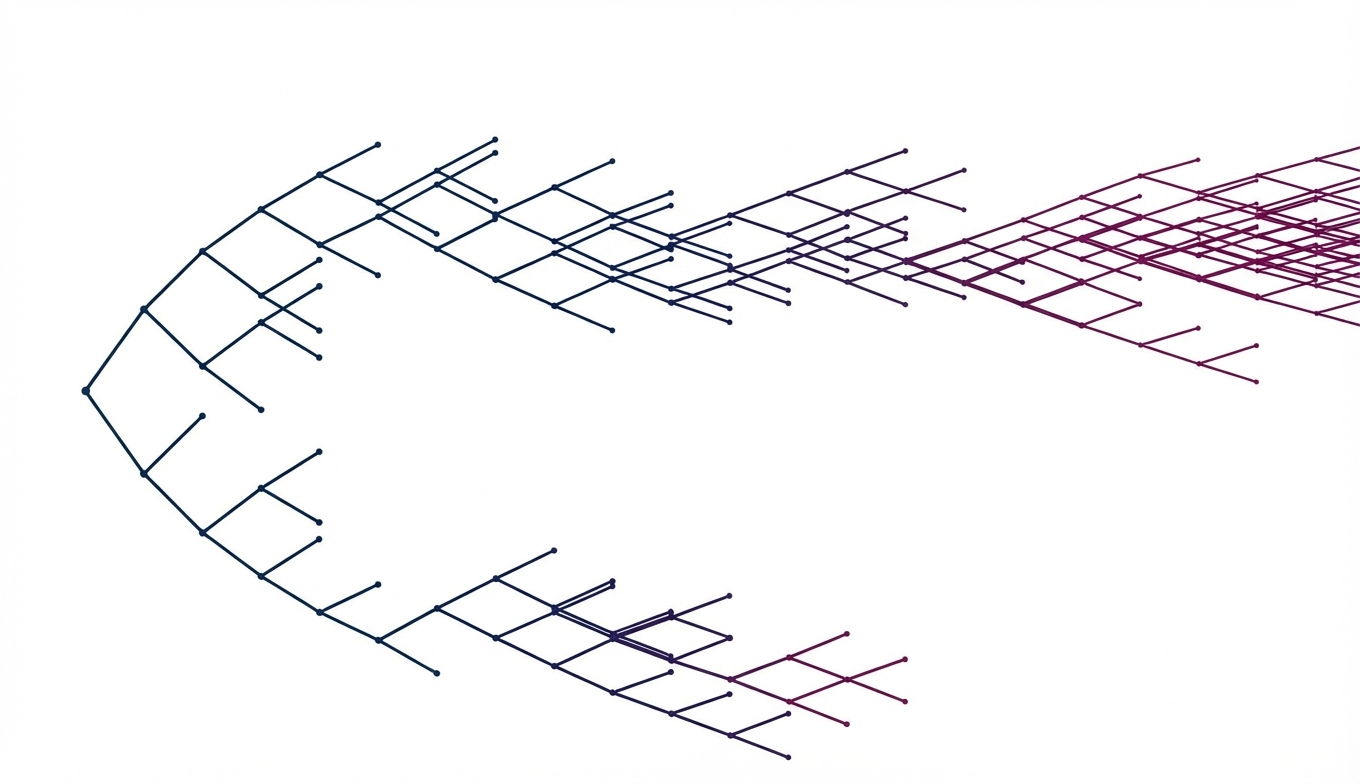
\includegraphics[width=0.78\textwidth]{figures/IMG_ch3/simpleGWvis.png}\\[6pt]
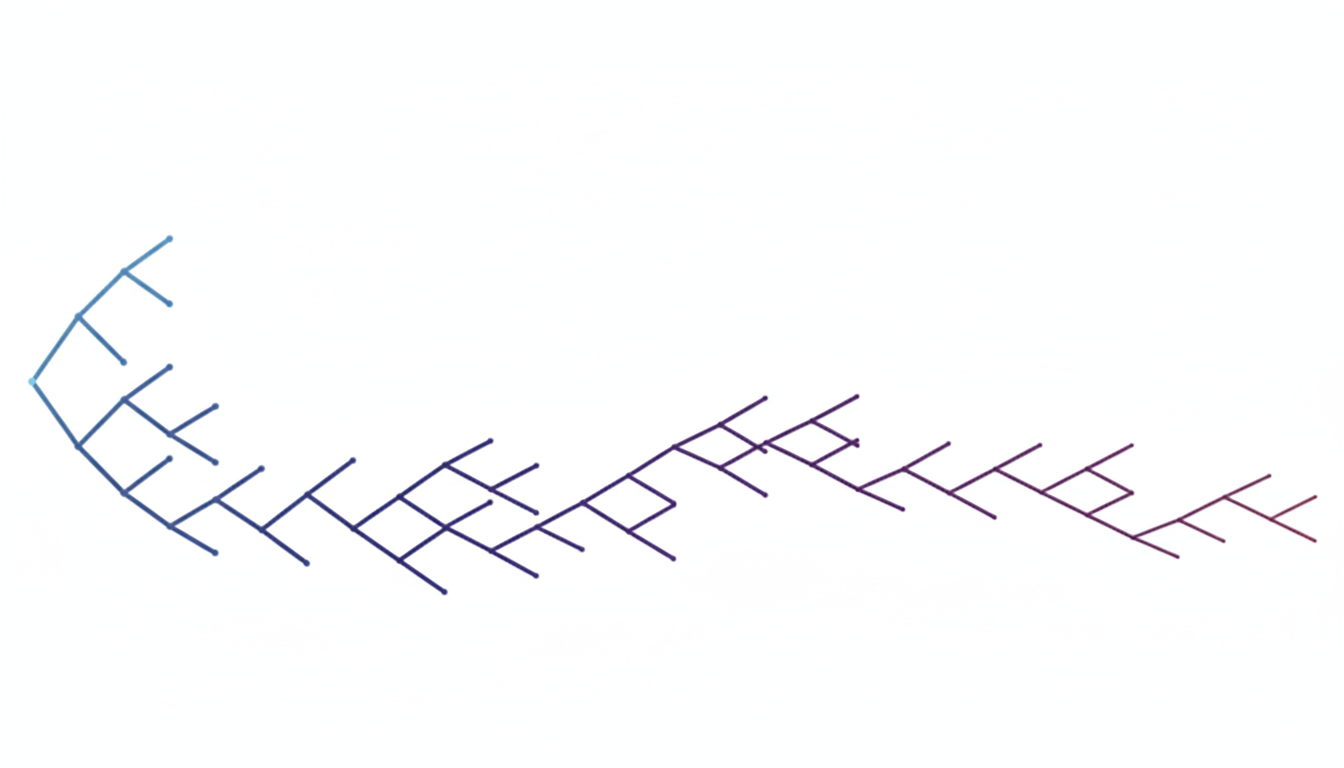
\includegraphics[width=0.78\textwidth]{figures/IMG_ch3/subGWvis.png}
\caption{Realisations of the simple Galton--Watson process, drawn as genealogies
with generation increasing to the right. Top: supercritical, $p=0.58$; the number of
lines grows without bound. Bottom: subcritical, $p=0.47$; the same construction, but
the tree terminates. Colour encodes generation number.}
\label{fig:gwvis}
\end{figure}

\noindent
The offspring \pgf{} is
\begin{equation}
\label{eq:pgfbinary}
\phi(z) = \mean{z^{\zz_1}} = p z^2 + (1-p),
\end{equation}
so that \cref{iterPGF} reads
\begin{equation}
\label{unIter}
u_{n+1} = p\,u_n^2 + 1-p .
\end{equation}
The recursion admits a direct reading. If the founder dies at its first step, which
happens with probability $1-p$, extinction has already occurred. If instead it
divides, with probability $p$, then extinction by generation $n+1$ requires each of
the two fresh lineages to die out within its own $n$ generations, which happens with
probability $u_n^2$.

It is more convenient to work with the complement,
\begin{equation*}
S_n = 1-u_n = \pr{\zz_n>0},
\end{equation*}
the probability that the process is still alive at generation $n$. Substituting
$u_n = 1-S_n$ into \cref{unIter} and simplifying gives
\begin{equation}
\label{SnIter}
S_{n+1} = 2p S_n - p S_n^2,\qquad S_0 = 1.
\end{equation}
Since a population cannot return from extinction, $u_n$ is non-decreasing and
bounded above by $1$; equivalently $S_n$ is non-increasing and bounded below by $0$,
and therefore converges to some $S_\infty\in[0,1]$.

\subsection{Certainty of extinction}
\label{sec:certainty}

Because $S_n$ converges, the limit must be a fixed point of \cref{SnIter}. Setting
$S_{n+1}=S_n=S_\infty$,
\begin{equation*}
S_\infty = 2p S_\infty - p S_\infty^2
\qquad\Longleftrightarrow\qquad
p\,S_\infty\bigl(S_\infty + \tfrac1p - 2\bigr) = 0,
\end{equation*}
whose roots are
\begin{equation*}
S_\infty = 0
\qquad\text{and}\qquad
S_\infty = 2 - \frac1p = \frac{2p-1}{p}.
\end{equation*}
For $p<\tfrac12$ the second root is negative and so carries no probabilistic
meaning; the only admissible limit is $S_\infty=0$ and extinction is certain. At
$p=\tfrac12$ the two roots collide at the origin, and extinction remains certain.
For $p>\tfrac12$ a positive root appears, $S_\infty = (2p-1)/p$, and it is this root
that is attained: the process survives forever with positive probability.
\Cref{fig:phase_transition} shows the transition.

\begin{figure}[htbp]
    \centering
    \begin{subfigure}[b]{0.31\textwidth}
        \centering
        \begin{tikzpicture}
            \begin{axis}[myplotstyle]
                \addplot[blue, thick] {2*0.3*x - 0.3*x^2};
                \addplot[black!45, dashed] {x};
                \addplot[only marks, mark=*, red, mark size=1.6pt] coordinates {(0,0)};
            \end{axis}
        \end{tikzpicture}
        \caption{Subcritical ($p = 0.3$)}
    \end{subfigure}
    \hfill
    \begin{subfigure}[b]{0.31\textwidth}
        \centering
        \begin{tikzpicture}
            \begin{axis}[myplotstyle]
                \addplot[blue, thick] {2*0.5*x - 0.5*x^2};
                \addplot[black!45, dashed] {x};
                \addplot[only marks, mark=*, red, mark size=1.6pt] coordinates {(0,0)};
            \end{axis}
        \end{tikzpicture}
        \caption{Critical ($p = 0.5$)}
    \end{subfigure}
    \hfill
    \begin{subfigure}[b]{0.31\textwidth}
        \centering
        \begin{tikzpicture}
            \begin{axis}[myplotstyle]
                \addplot[blue, thick] {2*0.74*x - 0.74*x^2};
                \addplot[black!45, dashed] {x};
                \addplot[only marks, mark=*, red, mark size=1.6pt] coordinates {(0,0) (0.64865,0.64865)};
            \end{axis}
        \end{tikzpicture}
        \caption{Supercritical ($p = 0.74$)}
    \end{subfigure}

    \vspace{10pt}
    \begin{subfigure}[b]{0.55\textwidth}
    \centering
    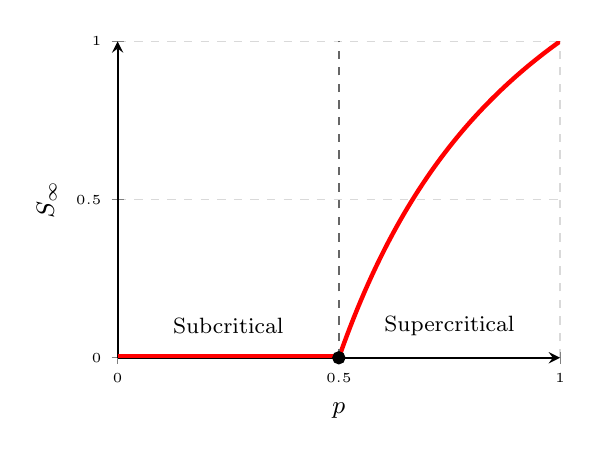
\begin{tikzpicture}
        \begin{axis}[
            width=7.2cm, height=5.6cm,
            axis lines=left,
            xlabel={$p$}, ylabel={$S_\infty$},
            xmin=0, xmax=1, ymin=0, ymax=1,
            xtick={0,0.5,1}, ytick={0,0.5,1},
            grid=major, grid style={dashed, gray!30}, thick,
            label style={font=\small}, tick label style={font=\tiny}
        ]
            \addplot[red, ultra thick, domain=0:0.5] {0.004};
            \addplot[red, ultra thick, domain=0.5:1, samples=120] {(2*x-1)/x};
            \draw[dashed, black!60] (axis cs:0.5,0) -- (axis cs:0.5,1);
            \node[font=\footnotesize] at (axis cs:0.25, 0.10) {Subcritical};
            \node[font=\footnotesize] at (axis cs:0.75, 0.10) {Supercritical};
            \addplot[only marks, mark=*, mark size=2pt, black] coordinates {(0.5,0)};
        \end{axis}
    \end{tikzpicture}
    \caption{The transition in $S_\infty$}
    \end{subfigure}

    \caption{Steady states of the survival recursion \cref{SnIter}. Panels (a)--(c)
    show the map $S\mapsto 2pS-pS^{2}$ (blue) against the diagonal (dashed); fixed
    points are the intersections, marked in red. Below and at criticality the origin
    is the only fixed point in $[0,1]$, and it is attracting, so extinction is
    certain. At $p=\tfrac12$ the map becomes tangent to the diagonal at the origin.
    For $p>\tfrac12$ the origin turns repelling and a stable positive fixed point
    $S_\infty=(2p-1)/p$ separates from it, traced in panel~(d). The survival
    probability is identically zero below the critical point and rises continuously
    above it.}
    \label{fig:phase_transition}
\end{figure}

\subsection{The critical case: a power law and an infinite expected lifetime}
\label{sec:criticalcase}

At $p=\tfrac12$ the expectation is constant, $\mean{\zz_n} = 1^n = 1$ for all $n$,
and yet extinction is certain. The reconciliation is that the expected
\emph{lifetime} is infinite: rare realisations survive for enormously long times and
grow enormously large, and they do so at exactly the rate needed to hold the mean at
one. This is worth demonstrating, because the same calculation supplies the
asymptotics of $S_n$ that \cref{sec:Ap} will need.

Let
\begin{equation*}
T = \inf\{n : \zz_n = 0\}
\end{equation*}
be the extinction time, so that the process passes through generations
$0,1,\dots,T-1$ and is dead at $T$. Writing $T$ as a sum of indicators,
\begin{equation*}
T = \sum_{n=0}^{\infty}\mathbf{1}_{\{T>n\}},
\end{equation*}
and taking expectations term by term (all terms are non-negative, so the exchange is
legitimate),
\begin{equation}
\label{eq:ETsumSn}
\mean{T} = \sum_{n=0}^{\infty}\pr{T>n} = \sum_{n=0}^{\infty}\pr{\zz_n>0} = \sum_{n=0}^{\infty}S_n .
\end{equation}
So the question becomes: how fast does $S_n$ go to zero at criticality?

Setting $p=\tfrac12$ in \cref{SnIter} gives $S_{n+1} = S_n - \tfrac12 S_n^2$, that is
\begin{equation*}
S_{n+1}-S_n = -\tfrac12 S_n^2 .
\end{equation*}
Once $n$ is large the unit generational increment is small compared with the scale
on which $S_n$ varies, and the difference on the left is well approximated by a
derivative:
\begin{equation*}
\frac{\dd S}{\dd n} = -\tfrac12 S^2,
\qquad\text{with general solution}\qquad
S(n) = \frac{2}{n + \text{const}}.
\end{equation*}
Hence
\begin{equation}
\label{twoovrn_sn}
S_n \sim \frac{2}{n}\qquad (n\to\infty),
\end{equation}
which the simulations of \cref{fig:power_law}(a) confirm. Substituting into
\cref{eq:ETsumSn}, the tail of the sum behaves like twice the harmonic series,
\begin{equation*}
\mean{T} = \sum_{n=0}^{\infty}S_n \sim \sum_{n=1}^{\infty}\frac{2}{n},
\end{equation*}
which diverges. Since every $S_n$ is positive, $\mean{T}=\infty$. The expected
lifetime of the critical Galton--Watson process is infinite even though extinction
occurs with probability one.

\begin{figure}[H]
    \centering
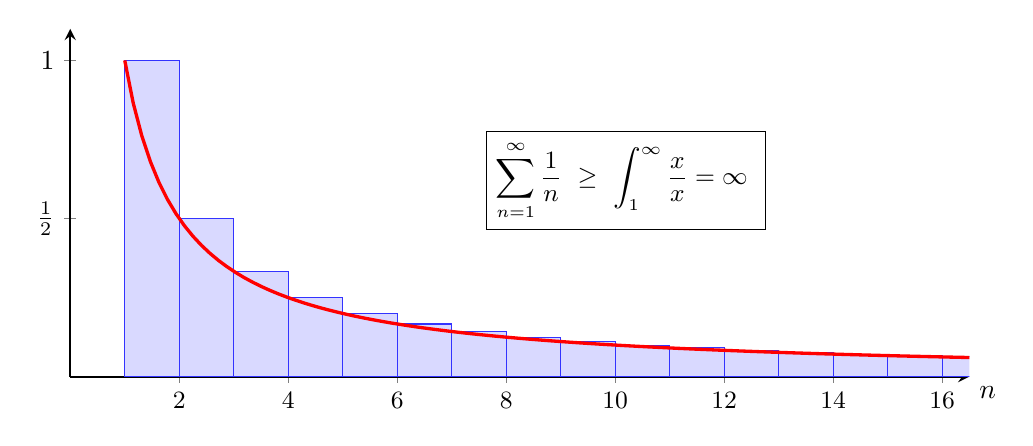
\begin{tikzpicture}
    \begin{axis}[
        axis lines = middle,
        xmin = 0, xmax = 16.5, ymin = 0, ymax = 1.1,
        xlabel = {$n$},
        xtick = {2,4,6,8,10,12,14,16},
        ytick = {0.5, 1}, yticklabels = {$\frac{1}{2}$, $1$},
        axis line style = {thick},
        width = 13cm, height = 6cm,
        every axis x label/.style={at={(current axis.right of origin)}, anchor=north west},
        xticklabel style={font=\small},
    ]
        \addplot[fill=blue!15, draw=blue!80, ybar interval, samples at={1,2,...,17}] {1/x} \closedcycle;
        \addplot[red, domain=1:16.5, samples=100, very thick] {1/x};
        \node[draw, fill=white, align=left, font=\small] at (axis cs: 10.2, 0.62) {
            $\displaystyle \sum_{n=1}^{\infty} \frac{1}{n} \ \ge\ \int_{1}^{\infty} \frac{\dd x}{x} = \infty$
        };
    \end{axis}
\end{tikzpicture}
\caption{Divergence of the harmonic series. Each blue rectangle has area $1/n$ and
contains the region under the red curve $1/x$ on $[n,n+1]$, so the sum of the areas
exceeds $\int_1^\infty x^{-1}\dd x = \infty$. Because $S_n\sim 2/n$ at criticality,
the same divergence carries over to $\mean{T}=\sum_n S_n$.}
\label{fig:harmonic}
\end{figure}

The heavy tail responsible for this is visible directly in simulation. For a
power-law distributed variable there is a modest but non-negligible chance of an
extraordinarily large realisation, and a sample mean computed from such a variable
does not settle: the larger the sample, the larger the mean, because the occasional
enormous value keeps pushing the normalised sum upward. \Cref{fig:power_law}
collects the three classical critical exponents.

\begin{figure}[ht]
    \centering
    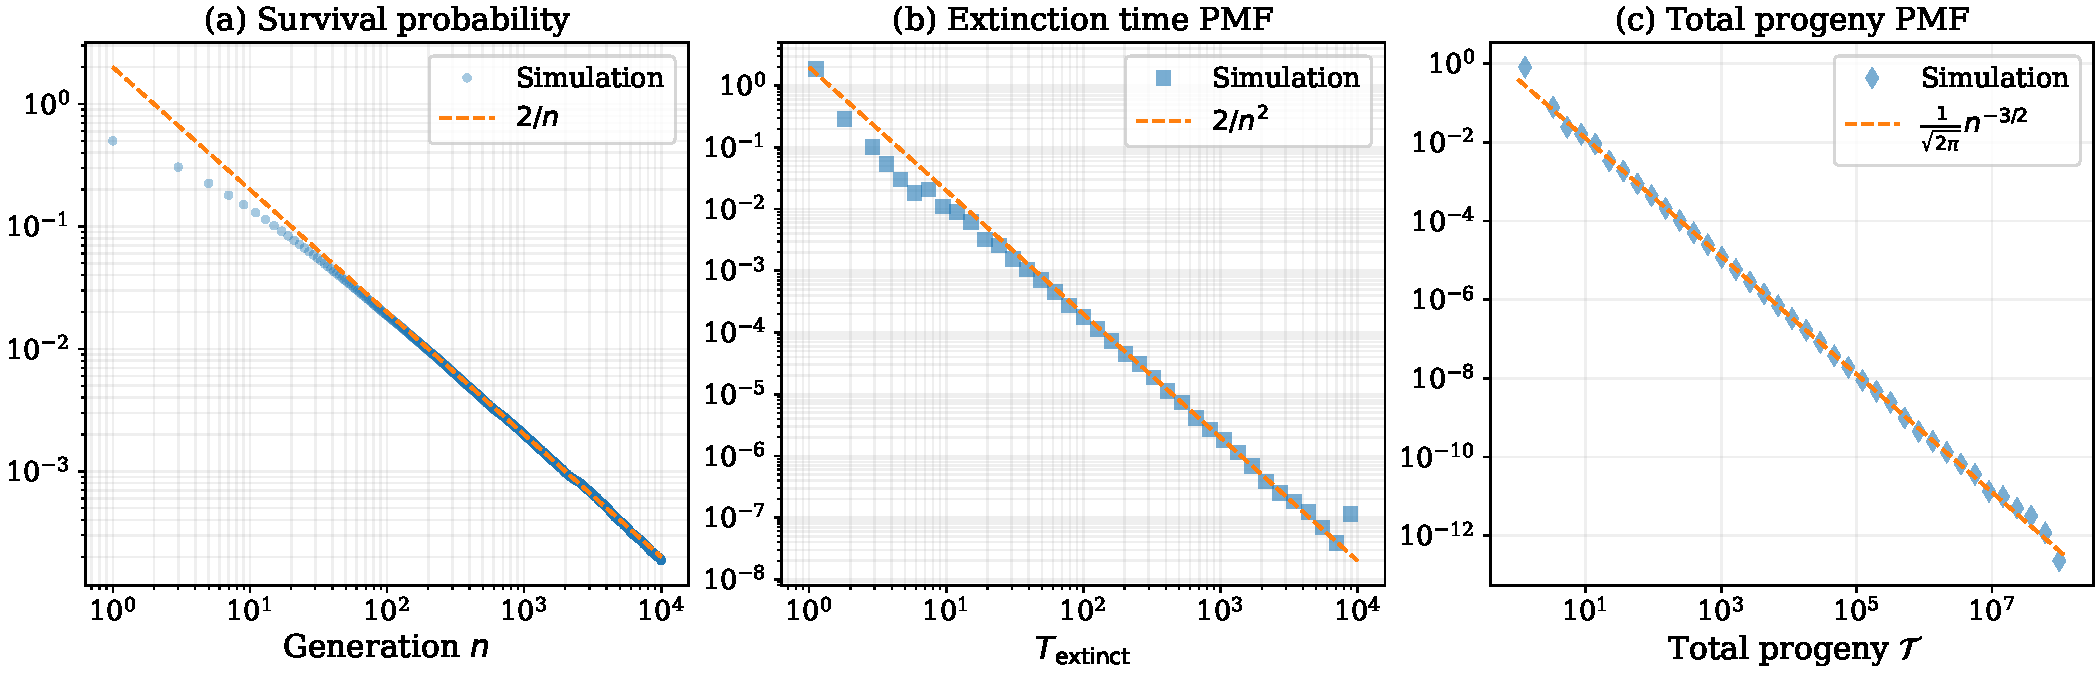
\includegraphics[width=0.98\textwidth]{figures/IMG_ch3/power_law_fixed.pdf}
    \caption{Power-law behaviour in the critical Galton--Watson process
    ($p=0.5$), from $10^6$ realisations.
    (a) Survival probability $S_n=\pr{\zz_n>0}$, showing the late-generation scaling
    $S_n \sim 2/n$ of \cref{twoovrn_sn}.
    (b) Probability mass function of the extinction time
    $T = \inf\{n : \zz_n = 0\}$, with heavy tail
    $\pr{T = n}\sim 2/n^{2}$.
    (c) Probability mass function of the total progeny
    $\mathcal{T} = \sum_{k\ge0}\zz_k$, displaying the classical critical branching
    asymptotic $\pr{\mathcal{T}=n}\sim n^{-3/2}$.}
    \label{fig:power_law}
\end{figure}

\FloatBarrier
